%% BioMed_Central_Tex_Template_v1.06
%%                                      %
%  bmc_article.tex            ver: 1.06 %
%                                       %

%%IMPORTANT: do not delete the first line of this template
%%It must be present to enable the BMC Submission system to
%%recognise this template!!

%%%%%%%%%%%%%%%%%%%%%%%%%%%%%%%%%%%%%%%%%
%%                                     %%
%%  LaTeX template for BioMed Central  %%
%%     journal article submissions     %%
%%                                     %%
%%          <8 June 2012>              %%
%%                                     %%
%%                                     %%
%%%%%%%%%%%%%%%%%%%%%%%%%%%%%%%%%%%%%%%%%


%%%%%%%%%%%%%%%%%%%%%%%%%%%%%%%%%%%%%%%%%%%%%%%%%%%%%%%%%%%%%%%%%%%%%
%%                                                                 %%
%% For instructions on how to fill out this Tex template           %%
%% document please refer to Readme.html and the instructions for   %%
%% authors page on the biomed central website                      %%
%% http://www.biomedcentral.com/info/authors/                      %%
%%                                                                 %%
%% Please do not use \input{...} to include other tex files.       %%
%% Submit your LaTeX manuscript as one .tex document.              %%
%%                                                                 %%
%% All additional figures and files should be attached             %%
%% separately and not embedded in the \TeX\ document itself.       %%
%%                                                                 %%
%% BioMed Central currently use the MikTex distribution of         %%
%% TeX for Windows) of TeX and LaTeX.  This is available from      %%
%% http://www.miktex.org                                           %%
%%                                                                 %%
%%%%%%%%%%%%%%%%%%%%%%%%%%%%%%%%%%%%%%%%%%%%%%%%%%%%%%%%%%%%%%%%%%%%%

%%% additional documentclass options:
%  [doublespacing]
%  [linenumbers]   - put the line numbers on margins

%%% loading packages, author definitions

%\documentclass[twocolumn]{bmcart}% uncomment this for twocolumn layout and comment line below
\documentclass{bmcart}
%  Recompile
%2


%%% Load packages
\usepackage{amsthm,amsmath}
\RequirePackage{natbib}
\usepackage{natbib}
\usepackage{graphicx}
\usepackage{subcaption}
\RequirePackage[authoryear]{natbib}% uncomment this for author-year bibliography
%\RequirePackage{hyperref}
\usepackage[utf8]{inputenc} %unicode support
%\usepackage[applemac]{inputenc} %applemac support if unicode package fails
%\usepackage[latin1]{inputenc} %UNIX support if unicode package fails
%\usepackage{natbib}

%%%%%%%%%%%%%%%%%%%%%%%%%%%%%%%%%%%%%%%%%%%%%%%%%
%%                                             %%
%%  If you wish to display your graphics for   %%
%%  your own use using includegraphic or       %%
%%  includegraphics, then comment out the      %%
%%  following two lines of code.               %%
%%  NB: These line *must* be included when     %%
%%  submitting to BMC.                         %%
%%  All figure files must be submitted as      %%
%%  separate graphics through the BMC          %%
%%  submission process, not included in the    %%
%%  submitted article.                         %%
%%                                             %%
%%%%%%%%%%%%%%%%%%%%%%%%%%%%%%%%%%%%%%%%%%%%%%%%%

%\def\includegraphic{}
%\def\includegraphics{}

%%% Put your definitions there:
\startlocaldefs
\endlocaldefs


%%% Begin ...
\begin{document}


%%% Start of article front matter
\begin{frontmatter}

\begin{fmbox}
\dochead{Research}

%%%%%%%%%%%%%%%%%%%%%%%%%%%%%%%%%%%%%%%%%%%%%%
%%                                          %%
%% Enter the title of your article here     %%
%%                                          %%
%%%%%%%%%%%%%%%%%%%%%%%%%%%%%%%%%%%%%%%%%%%%%%

\title{Prevalence and the variance of state occupancy time}

%%%%%%%%%%%%%%%%%%%%%%%%%%%%%%%%%%%%%%%%%%%%%%
%%                                          %%
%% Enter the authors here                   %%
%%                                          %%
%% Specify information, if available,       %%
%% in the form:                             %%
%%   <key>={<id1>,<id2>}                    %%
%%   <key>=                                 %%
%% Comment or delete the keys which are     %%
%% not used. Repeat \author command as much %%
%% as required.                             %%
%%                                          %%
%%%%%%%%%%%%%%%%%%%%%%%%%%%%%%%%%%%%%%%%%%%%%%

\author[
   addressref={aff1},                   % id's of addresses, e.g. {aff1,aff2}
   corref={aff1},                       % id of corresponding address, if any
   noteref={n1},                        % id's of article notes, if any
   email={riffe@demogr.mpg.de}   % email address
]{\inits{TR}\fnm{Tim} \snm{Riffe}}
%\author[
%   addressref={aff1,aff2},
%   email={john.RS.Smith@cambridge.co.uk}
%]{\inits{JRS}\fnm{John RS} \snm{Smith}}

%%%%%%%%%%%%%%%%%%%%%%%%%%%%%%%%%%%%%%%%%%%%%%
%%                                          %%
%% Enter the authors' addresses here        %%
%%                                          %%
%% Repeat \address commands as much as      %%
%% required.                                %%
%%                                          %%
%%%%%%%%%%%%%%%%%%%%%%%%%%%%%%%%%%%%%%%%%%%%%%

\address[id=aff1]{%                           % unique id
  \orgname{Max-Planck-Institute for Demographic Research}, % university, etc
  \street{Konrad-Zuse-Str. 1},                     %
  \postcode{18057}                                % post or zip code
  \city{Rostock},                              % city
  \cny{Germany}                                    % country
}

%%%%%%%%%%%%%%%%%%%%%%%%%%%%%%%%%%%%%%%%%%%%%%
%%                                          %%
%% Enter short notes here                   %%
%%                                          %%
%% Short notes will be after addresses      %%
%% on first page.                           %%
%%                                          %%
%%%%%%%%%%%%%%%%%%%%%%%%%%%%%%%%%%%%%%%%%%%%%%

\begin{artnotes}
\note{This manuscript is in its early stages}     % note to the article
\note[id=n1]{~} % note, connected to author
\end{artnotes}

\end{fmbox}% comment this for two column layout

%%%%%%%%%%%%%%%%%%%%%%%%%%%%%%%%%%%%%%%%%%%%%%
%%                                          %%
%% The Abstract begins here                 %%
%%                                          %%
%% Please refer to the Instructions for     %%
%% authors on http://www.biomedcentral.com  %%
%% and include the section headings         %%
%% accordingly for your article type.       %%
%%                                          %%
%%%%%%%%%%%%%%%%%%%%%%%%%%%%%%%%%%%%%%%%%%%%%%

\begin{abstractbox}

\begin{abstract} % abstract
\parttitle{Background} 
Markov reward methods have been proposed to calculate the variance of state occupancy time based on age-structured prevalence and survivorship.
\parttitle{Objectives} I aim to clarify the assumptions of this approach, give bounds to its reasonableness, and suggest improvements.
\parttitle{Methods} I calculate results for extreme cases to provide bounds, I simulate the variance under simple assumptions, and simulate a more natural inter-individual state distribution.
\parttitle{Results} I show that state occupancy variance for Sullivan-style inputs is not identified, and I show where previously proposed methods fall with respect to reasonable bounds, randomly generated variances, and my own opinion about what a reasonable inter-individual state distribution might look like.
\parttitle{Conclusions} 
The variance of state occupancy time is only identified if a) state life trajectories are directly observed or b) a process model, such as an incidence-based Markov model, is specified. Sullivan-calculations of life expectancy do not imply a single variance, and are therefore insufficient to make statements on inter-individual disparities in state occupancies.
\end{abstract}

%%%%%%%%%%%%%%%%%%%%%%%%%%%%%%%%%%%%%%%%%%%%%%
%%                                          %%
%% The keywords begin here                  %%
%%                                          %%
%% Put each keyword in separate \kwd{}.     %%
%%                                          %%
%%%%%%%%%%%%%%%%%%%%%%%%%%%%%%%%%%%%%%%%%%%%%%

\begin{keyword}
\kwd{Healthy life expectancy}
\kwd{Sullivan method}
\kwd{Healthy life variance}
\end{keyword}

% MSC classifications codes, if any
%\begin{keyword}[class=AMS]
%\kwd[Primary ]{}
%\kwd{}
%\kwd[; secondary ]{}
%\end{keyword}

\end{abstractbox}
%

%\end{fmbox}% uncomment this for twcolumn layout

\end{frontmatter}

%%%%%%%%%%%%%%%%%%%%%%%%%%%%%%%%%%%%%%%%%%%%%%
%%                                          %%
%% The Main Body begins here                %%
%%                                          %%
%% Please refer to the instructions for     %%
%% authors on:                              %%
%% http://www.biomedcentral.com/info/authors%%
%% and include the section headings         %%
%% accordingly for your article type.       %%
%%                                          %%
%% See the Results and Discussion section   %%
%% for details on how to create sub-sections%%
%%                                          %%
%% use \cite{...} to cite references        %%
%%  \cite{koon} and                         %%
%%  \cite{oreg,khar,zvai,xjon,schn,pond}    %%
%%  \nocite{smith,marg,hunn,advi,koha,mouse}%%
%%                                          %%
%%%%%%%%%%%%%%%%%%%%%%%%%%%%%%%%%%%%%%%%%%%%%%

\section*{Introduction}
Health inequality is usually measured between populations by comparing life expectancies, health expectancies, or poor health expectancies. Within populations there is also inequality in health outcomes, either due to violations of the assumption of homogeneity of risk sets or due to random variation between people otherwise subject to the same risk. The life table and related statistics typically assume homogeneity of age trajectories of risk between individuals, and multistate models assume the same within states. However, people can't seem to agree on how useful transition-based models are at producing reality. While most practitioners produce estimates with the Sullivan method \citep{sullivan1971single} becuse it is often the only viable option, but some Markov skeptics accept the simpler Sullivan method despite its flaws due its process-free interpretation. For the present, let's take the Sullivan estimate of life expectancy for granted and instead focus on within-population estimates of the variance of state occupancy time implied by the same data inputs. 

In this paper I will argue that no single variance is implied, that in fact infinitely many variances are possible under minimal Sullivan constraints. Instead further assumptions are required to constrain as necessary and arrive at variance calculations. Two such approaches are available assuming that variance results from 1) a discrete time Bernoulli process and 2) from prevalence as a fixed property within age \citep{caswell2018matrix}. I'll first translate these two present approaches to a more familair demographic notation, and illustrate their implications with a worked example. I'll argue that neither of these approaches reflects health prevalence patterns particularly well, and that instead ut then give my own best approximation of Sullivan variance given what we know about how health processes work. This is at best a hackish patch for an otherwise intractable problem, but we will make the best use of some stationary population properties and some observations of incidence-prevalence relationships to give some hopefully-useful rules of thumb. 

At best these rules of thumb will stimulate further efforts to improve them into something that might be adopted in practice, although it would also be a perfectly good outcome if practitioners simply withheld from calculating the variance of state occupancy for Sullivan (health) inputs unless the health process and available approximations are well understood and judged apt. Presently available methods may indeed be apt in other domians.



\section*{Sullivan in continuous time}
Let's begin with some familiar notation, $\ell(x)$ denotes lifetable survivorship, with an arbitrary radix, or starting population. If $\ell(0) = 1$ then $\ell(x)$ can be interpreted as a probability of surviving from birth until age $x$. $\pi(x)$ is the prevalence of a given condition (healthiness or unhealthiness, disability) at age $x$, and it falls in the range $[0,1]$, giving it a probability interpretation. The commonly used Sullivan method \citep{sullivan1971single} of calculating healthy life expectancy, $e^H(x)$ is to integrate the product of these two functions.
%
\begin{equation}
\label{eq:sull}
e^H(x) = \frac{1}{\ell(x)} \int_x^\omega \ell(t)\pi(t) \mathrm{d}t
\end{equation}
%

Replace $\pi$ with its complement to arrive at the complementary expectancy, $e^U(x)$, such that overall life expectancy for this age is $e(x) = e^U(x) + e^H(x)$, a rudimentary composition. Throughout this exposition, and for the sake of comparing methods, I'll stick to an odd choice of discretization of \ref{eq:sull}, which assume that an age entered is an age fully lived, i.e., that an age entered is a reward earned. For the case of \eqref{eq:sull}, this translates to:
\begin{equation}
\label{eq:sulldisc}
e^H(x) = \frac{1}{\ell_x} \sum_{t=x}^\omega \ell_t\pi_t \quad \mathrm{,}
\end{equation}
where subscripts denote the lower bound of the age interval, and function values are assumed constant through the interval. Age intervals are omitted from notation throughout for clarity. Undernormal circumstances, one would prefer to replace $\ell_x$ inside the summation with $L_x$ to account for attrition over the course of the year, but we resist this temptation to keep comparisons simple.

\section*{Two assumptions}
If we would like to know something about the variance of state occupancy in a Sullivan setup, then we must make some assumptions about how the state is distributed over individuals. The Sullivan method does not state which between-individual state distribution underlies prevalence in a given age. If $\pi(x) = 0.5$, shall we assign each individual age $x$ a value of 0.5 a so-called \emph{fixed reward}, or shall we assign half of them a value of 1, and the other half a value of 0, a \emph{Bernoulli reward} \citep{caswell2018matrix}? Or something else entirely? There are infinitely many ways to distribute state $\pi$ among individuals in age $x$ such that the value $\pi(x)$ is maintained. By extension, the inter-individual distribution of total time spent in state $\pi$ is also infinitely variable, which implies that the variance and other moments of implied state occupancy are not uniquely identified. 

Expressing the lifetable as a Markov chain with \emph{rewards} defined as prevalence gives a unique definition for the variance of state occupancy for each of the above assumptions, but it is unclear to me how well-supported these are. Many other reward types are discussed by Caswell \& Zarulli \cite{caswell2018matrix}, and I do not discuss these, nor do I treat the case of multistate populations. Even so, the conclusions reached here will generalize to the case of multistate populations.

%We will use two shorthand and equivalent forms to calculate variance, depending on the situation. First the mean of the squared residuals:
%\begin{equation}
%Var(X) = \mathbb{E}\left[(X-\mathbb{E}[X])^2 \right] \quad \mathrm{,}
%\end{equation}
%where in practice the outer expectation is taken as the sum of the squared residuals duly weighted by their respective probabilities of ocurring. The second is

\subsection*{Bernoulli rewards}
I'll first give my own lifetable deconstruction of the matrix algebra approach given to Bernoulli state variance in \cite{caswell2018matrix}. Then $e^H(x)$ is defined per \eqref{eq:sull}, and it is the first moment of state occupancy, which we can denote $\eta^{(1)}$, where the superscript in parentheses denotes the moment number and is not a power. We continue to calculate the second moment of state occupancy, $\eta^{(2)}$ as:
\begin{equation}
\label{eq:bern2}
\eta^{(2)}_x = \frac{1}{\ell_x} \sum_{t=x}^\omega \ell_t\left[\pi_t + 2(1-q_t)\pi_t\eta^{(1)}_t\right] \quad \mathrm{,}
\end{equation}
where $q_x$ is the probability of death in the interval and $\omega$ is the highest age of death. Here notation omits intervals, but we assume to be working in discrete bins of uniform width, where death and transition changes only happen in the moment of interval steps, implying a stepped survival curve and discrete life trajectories. We also assume that the same prevalence applies to each length-of-life bin within each age, ergo that all other unmodeled population strata have the same prevalence. Then the variance is determined, and it can be calculated as:
\begin{equation}
\label{eq:var2}
Var_x = \eta^{(2)}_x - (\eta^{(1)}_x)^2
\end{equation}

I highlight two assumptions behind this expression: 1) mortality is independent of whether one is in the prevalent state, and 2) the same Bernoulli prevalence extends to any further stratification of the members in a given age class, $x$.

\subsection*{Fixed rewards}
If instead of assuming that prevalence is partitioned in a binary fashion, and each individual experiences $\pi_x$ fraction of the year in the state, then equation \eqref{eq:bern2} becomes
\begin{equation}
\eta^{(2)}_x = \frac{1}{\ell_x} \sum_{t=x}^\omega \ell_t\left[\pi_t^2 + 2(1-q_t)\pi_t\eta^{(1)}_t\right] \quad \mathrm{,}
\end{equation}
and \eqref{eq:var2} is the same. State occupancy variance under the assumption of fixed rewards also has a more intuitive lifetable expression:
\begin{equation}
\label{eq:varfixed2}
Var_x = \frac{1}{l_x}\sum_x^\omega (\mathcal{P}_t - \eta^{(1)}_x)^2 d_t \quad\mathrm{,}
\end{equation}
where $\mathcal{P}_t$ is the cumulative prevalence from age $x$ to age $t$, and $d_t$ is the probability of survival from age $x$ to age $t$, defined as $(q_t l_t)/l_x$. 
\section{Illustrations of Bernoulli and fixed prevalence}
To add intuition to the previous equations I give a worked example of manageable size. Define a population with three discrete age groups of uniform width 1, and assume that state transitions occur only on birthdays (this is relaxable). The prevalent state, say sickness, is coded with 1, whereas its complement is coded with 0. Then all 14 possible life trajectories are given in Fig.~\ref{fig:b1}. Some prevalence $\pi_x$, its complement, and some lifetable functions are given in Tab~\ref{tab:toy}.

\begin{table}[ht!]
\begin{tabular}{r|ccccl}
age & $\pi_x$ & $1-\pi_x$ & $l_x$ & $d_x$ & $q_x$\\
\hline
0 & 0.1 & 0.9 & 1.0 & 0.2 & 0.2   \\
1 & 0.5 & 0.5 & 0.8 & 0.5 & 0.625 \\
2 & 0.7 & 0.3 & 0.3 & 0.3 & 1.0  
\end{tabular}
\caption{Parameters for toy examples}
\label{tab:toy}
\end{table}

\subsection{Bernoulli illustration}
Fig.~\ref{fig:b1} imputes values of $\pi_x$ and $1-\pi_x$ from Tab~\ref{tab:toy} into their respective positions for all 14 possible discrete life trajectories. The product of the proportions in each life sequence
gives the probability of experiencing the given sequence of states conditional on total length of life. Fig~.~\ref{fig:b3} shows the same sequences, where height is scaled to the length-of-life conditional probability of observing the trajectory. The set of sequence probabilities within each length-of-life bin sum to 1, and this is why Fig~.~\ref{fig:b3} forms a set of even steps, each of height 1. These probabilities are not the probabilities-at-birth of observing the given sequence; for this the conditional probability of each sequence must be multiplied by the probability of surviving the respective length of time, in our case given by $d_x$ in Tab.~\ref{tab:toy}. For example, the probability of the 14th trajectory is given by $0.1\times 0.5\times 0.7\times 0.3 = 0.0105$
\begin{figure}
    \centering
    \begin{subfigure}[b]{0.4\textwidth}
        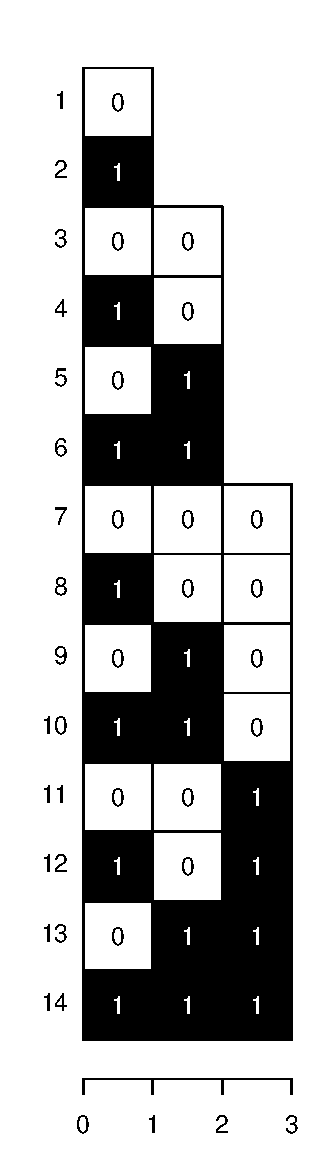
\includegraphics[scale=.5]{Figures/BernTraj.pdf}
        \caption{The binary 2-state trajectory space.}
        \label{fig:b1}
    \end{subfigure}
    ~ 
    \begin{subfigure}[b]{0.4\textwidth}
        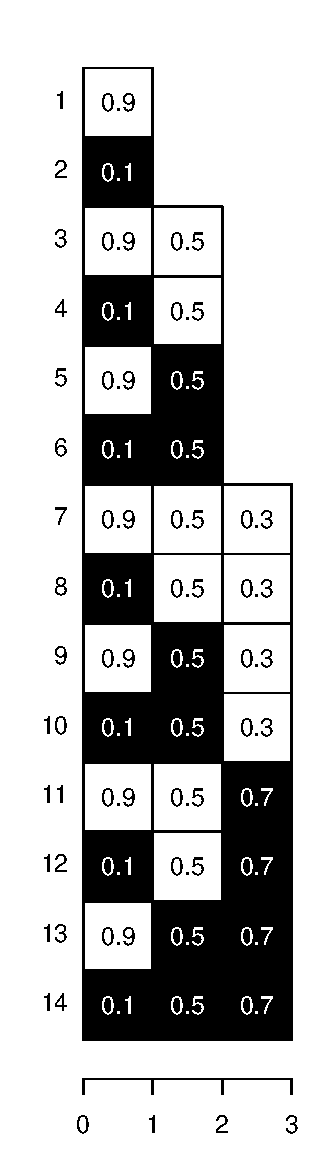
\includegraphics[scale=.5]{Figures/BernTrajProbs.pdf}
        \caption{With Bernoulli prevalence cell probabilities.}
        \label{fig:b2}
    \end{subfigure}
    
     \begin{subfigure}[b]{0.4\textwidth}
        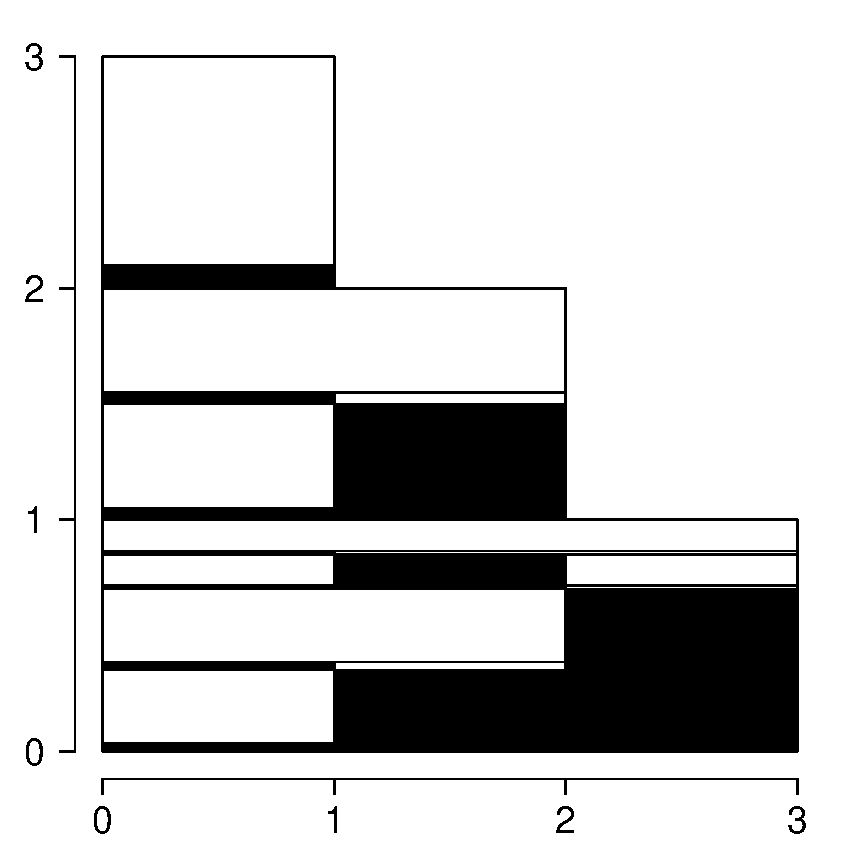
\includegraphics[scale=.4]{Figures/BernCondTrajProbs.pdf}
        \caption{With trajectories Bernoulli weighted, conditional on length of life.}
        \label{fig:b3}
    \end{subfigure}
    ~ 
    \begin{subfigure}[b]{0.4\textwidth}
        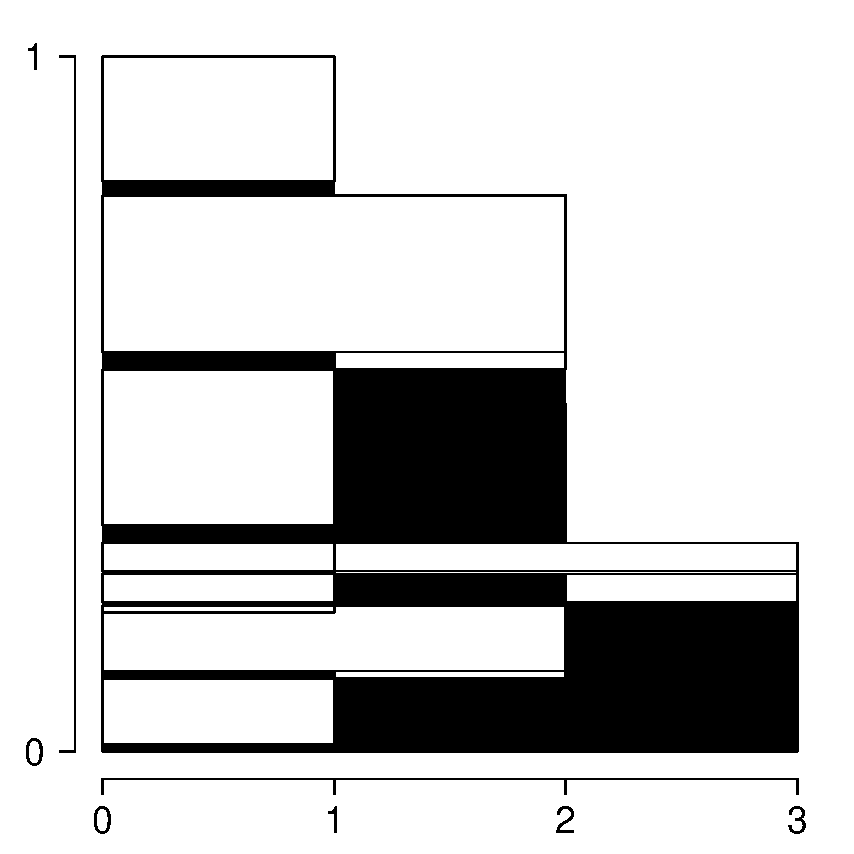
\includegraphics[scale=.4]{Figures/BernTrajProbsWeighted}
        \caption{With trajectories Bernoulli and lifetable weighted.\\}
        \label{fig:b4}
    \end{subfigure}
    \caption{A depiction of the Bernoulli life trajectories implied by the prevalence and lifetable of Tab.~\ref{tab:toy}. \ref{fig:b1} shows all binary discrete life sequences that are possible under these conditions. \ref{fig:b2} shows the conditional cell probabilities as drawn from $\pi_x$ and $1-\pi_x$ in Tab.~\ref{tab:toy}. \ref{fig:b3} shows the same sequences where height is defined as the probability of observing the sequence conditional on eventual length of life. \ref{fig:b4} shows the same sequences duly weighted by the length of life distribution $d_x$. This is the stationary sequence distribution implied by the discrete Bernoulli process of Tab.~\ref{tab:toy}. }\label{fig:bernexplain}
\end{figure}

The stationary sequence distribution depicted in Fig.~\ref{fig:b4} underlies the occupancy time distribution implied by our Bernoulli prevalence example. The heights of each sequence in this graph give the weights to assign to each trajectory, the item we wish to weight is the total number of black boxes per trajectory in Fig~\ref{fig:b1}, which gives the total time spent in the state of interest. For example, three of the trajectories (1,3,7) do not include time spent in the state, and only one of the sequences (14) consists in three years spent in the state. Fig.~\ref{fig:DiDist} shows the stationary distribution of state occupancy, with contributions from each trajectory stacked and indicated with labelled tick marks. This distribution gives an alternate path to the expectation of state occupancy of \eqref{eq:sull} and the variance of \eqref{eq:var2}. 
\begin{figure}[ht!]
\centering
\includegraphics[scale=.6]{Figures/DiDist_Ink.pdf}
\caption{The distribution of occupancy time defined by a Bernoulli interpretation of the prevalence and lifetable given in Tab.~\ref{tab:toy}. The height of each segment gives the proportion of lives the experience the total time given on the $x$ axis. Sub-segments indicated with labelled tick marks indicate the contributions from each sequence in Fig.~\ref{fig:bernexplain}.}\label{fig:DiDist}
\end{figure}

In our case the expectation at birth of time spent in the state is 0.71 years under Bernoulli prevalence assumptions, and the variance is 0.5379. These are identical results to those obtained from the matrix methods of \cite{caswell2018matrix} if one assumes that a full reward is assigned on entrance into an age/state.

\subsection{Fixed reward illustration}
We can also recycle values from Tab~\ref{tab:toy} to illustrate the meaning of fixed rewards. In this case $\mathcal{P}$ obtains the values $[0.1,0.6,1.3]$, and $d_x$ are our weights used to average these, giving us the same expectation of 0.71 years, but \eqref{eq:varfixed2} implies a variance of $0.1849$, quite different from the Bernoulli assumption. Under fixed rewards, one might redraw Fig.~\ref{fig:b4} as of a 2d uniform distribution under $l_x$ and within age bins, as in Fig.~\ref{fig:c1}, or else as binary year fractions, as in Fig.~\ref{fig:c2}. Indeed there are infinitely many ways to satisfy the constraints of fixed rewards by moving prevalence mass around within horizontal strips of age bins for this discrete case. Key for this case is that the cumulative value along any horizontal bisection is identical on birthday transitions.

\begin{figure}
\centering
    \begin{subfigure}[b]{0.4\textwidth}
        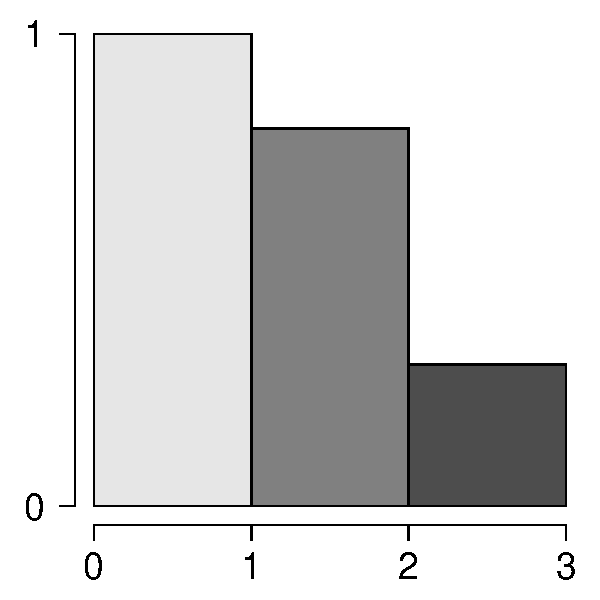
\includegraphics[scale=.5]{Figures/fixedflat.pdf}
        \caption{Fixed rewards uniformly distributed within age classes.}
        \label{fig:c1}
    \end{subfigure}
    ~ 
    \begin{subfigure}[b]{0.4\textwidth}
        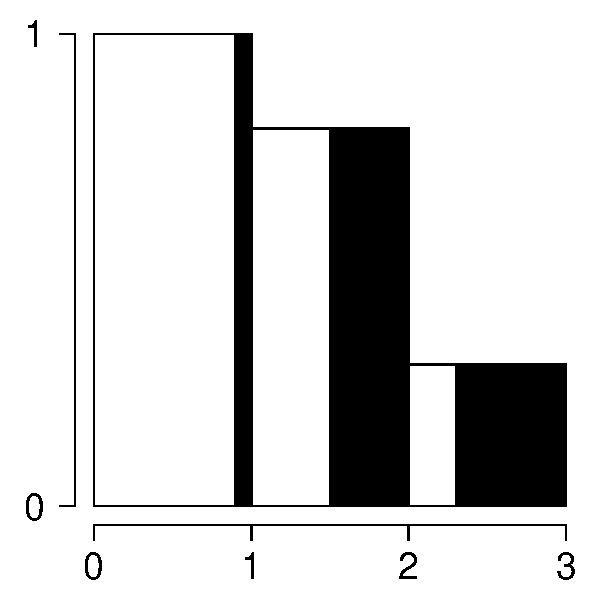
\includegraphics[scale=.5]{Figures/fixedbars.pdf}
        \caption{Fixed rewards as identical binary bands within age classes.}
        \label{fig:c2}
    \end{subfigure}
    \caption{Two interpretations of fixed rewards following the data of Tab.~\ref{tab:toy}. In Fig.~\ref{fig:c1} grayscale is proportional to the prevalence value, and in Fig.~\ref{fig:c2} the state is binary but assigned to an equal fraction of the year within age classes. There are also infinitely may ways to distribute states within age classes such that the same fraction is held}
    \label{fig:fixedexplain}
\end{figure}

\section{Alternative prevalence scenarios and their variances}
The purpose of 

%\nocite{oreg,schn,pond,smith,marg,hunn,advi,koha,mouse}

%%%%%%%%%%%%%%%%%%%%%%%%%%%%%%%%%%%%%%%%%%%%%%
%%                                          %%
%% Backmatter begins here                   %%
%%                                          %%
%%%%%%%%%%%%%%%%%%%%%%%%%%%%%%%%%%%%%%%%%%%%%%

\begin{backmatter}

\section*{Competing interests}
  The authors declare that they have no competing interests.

\section*{Author's contributions}
    TR did everything so far.

\section*{Acknowledgements}
  Thanks to Douglas Wolf and Jennifer Karas Montez for posing a question that led to this work, and to Hal Caswell and Virginia Zarulli for the groundwork on which this is based and for fielding inquiries.
%%%%%%%%%%%%%%%%%%%%%%%%%%%%%%%%%%%%%%%%%%%%%%%%%%%%%%%%%%%%%
%%                  The Bibliography                       %%
%%                                                         %%
%%  Bmc_mathpys.bst  will be used to                       %%
%%  create a .BBL file for submission.                     %%
%%  After submission of the .TEX file,                     %%
%%  you will be prompted to submit your .BBL file.         %%
%%                                                         %%
%%                                                         %%
%%  Note that the displayed Bibliography will not          %%
%%  necessarily be rendered by Latex exactly as specified  %%
%%  in the online Instructions for Authors.                %%
%%                                                         %%
%%%%%%%%%%%%%%%%%%%%%%%%%%%%%%%%%%%%%%%%%%%%%%%%%%%%%%%%%%%%%

% if your bibliography is in bibtex format, use those commands:
\bibliographystyle{bmc-mathphys} % Style BST file (bmc-mathphys, vancouver, spbasic).
\bibliography{references}      % Bibliography file (usually '*.bib' )
% for author-year bibliography (bmc-mathphys or spbasic)
% a) write to bib file (bmc-mathphys only)
% @settings{label, options="nameyear"}
% b) uncomment next line
%\nocite{label}

% or include bibliography directly:
% \begin{thebibliography}
% \bibitem{b1}
% \end{thebibliography}

%%%%%%%%%%%%%%%%%%%%%%%%%%%%%%%%%%%
%%                               %%
%% Figures                       %%
%%                               %%
%% NB: this is for captions and  %%
%% Titles. All graphics must be  %%
%% submitted separately and NOT  %%
%% included in the Tex document  %%
%%                               %%
%%%%%%%%%%%%%%%%%%%%%%%%%%%%%%%%%%%

%%
%% Do not use \listoffigures as most will included as separate files

%\section*{Figures}
%  \begin{figure}[h!]
%  \caption{\csentence{Sample figure title.}
%      A short description of the figure content
%      should go here.}
%      \end{figure}

%\begin{figure}[h!]
%  \caption{\csentence{Sample figure title.}
%      Figure legend text.}
%      \end{figure}

%%%%%%%%%%%%%%%%%%%%%%%%%%%%%%%%%%%
%%                               %%
%% Tables                        %%
%%                               %%
%%%%%%%%%%%%%%%%%%%%%%%%%%%%%%%%%%%

%% Use of \listoftables is discouraged.
%%
%\section*{Tables}
%\begin{table}[h!]
%\caption{Sample table title. This is where the description of the table should
% go.}
%      \begin{tabular}{cccc}
%        \hline
%           & B1  &B2   & B3\\ \hline
%        A1 & 0.1 & 0.2 & 0.3\\
%        A2 & ... & ..  & .\\
%        A3 & ..  & .   & .\\ \hline
%      \end{tabular}
%\end{table}

%%%%%%%%%%%%%%%%%%%%%%%%%%%%%%%%%%%
%%                               %%
%% Additional Files              %%
%%                               %%
%%%%%%%%%%%%%%%%%%%%%%%%%%%%%%%%%%%

\section*{Additional Files}
  \subsection*{Additional file 1 --- Sample additional file title}
    Additional file descriptions text (including details of how to
    view the file, if it is in a non-standard format or the file extension).  This might
    refer to a multi-page table or a figure.

  \subsection*{Additional file 2 --- Sample additional file title}
    Additional file descriptions text.


\end{backmatter}
\end{document}
